\documentclass{beamer}

\usepackage[font=small,labelfont=bf]{caption}
\usepackage{longtable}
\usepackage{subfiles}
\usepackage{subfig}
\usepackage{booktabs}
\setlength{\tabcolsep}{6pt}
% \usepackage[table]{xcolor}
\title{Dual Optimization for Newsvendor-like Problem}
% \title{Dual Method for Solving Flight Mainte0.00ce Scheduling Problem}
\author{Chuwen}
\date{\today}

\begin{document}
\frame{\titlepage}



\begin{frame}
  \frametitle{FMP: variant case and weighted summation}
  \begin{align}
    \label{eq:fmp.obj}  f = & \min_{x_{it}, u_{it}, \delta_t, \epsilon_t}
    \textcolor{red}{b}^\mathsf{T}  \delta + \textcolor{red}{h}^\mathsf{T}\epsilon                                   \\
    \nonumber \mathbf{s.t.} &                                                                                       \\
    \label{eq:fmp.demand}   & \sum_i \textcolor{red}{c_i} u_{it} + \delta_t - \epsilon_t = d_t,\quad\forall t \in T \\
                            & U_{i, \cdot}, S_{i, \cdot}, X_{i, \cdot} \in \Omega_i,\quad \forall i\in I
  \end{align}
  \begin{itemize}
    \item \(b, h\) are time-variant
    \item \(c_i \neq 1\).
  \end{itemize}
\end{frame}


\begin{frame}
  \frametitle{FMP: Lagrangian relaxation}
  For the FMP, dual function:
  \[\begin{aligned}
      \phi(\lambda) & = - \sum_t \lambda_t d_t + \sum_i  \min_{\Omega_i} \textcolor{red}{c_i} \sum_t \lambda_t u_{it} \\
    \end{aligned}\]

  It reduces to a set of low dimensional minimization problems for each \(i \in I, \forall \lambda\)

  (Recall \(\lambda_t \in [-b, h] \) and \(\delta_t^\star = \epsilon_t^\star = 0\) else unbounded)
  \begin{equation}\label{subproblem}\begin{aligned}
      \min_{\Omega_i} \textcolor{red}{c_i} \sum_t \lambda_t \cdot u_{i,t}
    \end{aligned}\end{equation}
  \eqref{subproblem} is the subproblem to be solved by dynamic programming. (states: lifespan, action: work or start maintence)
\end{frame}

\begin{frame}
  \frametitle{FMP: subgradient method}
  At each iteration \(k\):
  \begin{itemize}
    \item  \(y_k\) solves \(\phi(\lambda_k) = \min_y \lambda_k^\mathsf{T}(y-b)\)
    \item for FMP: \(y_k = U_k ^\mathsf{T} \textcolor{red}{c}, U_k = (u^{(k)}_{it})\), solved from \eqref{subproblem} by DP.
    \item update \(\lambda_k\).
  \end{itemize}
\end{frame}
\begin{frame}
  \frametitle{Small case: \(|I| = 1, t = 2\) }
  \begin{align*}
    \textcolor{red}{c = 1} &                                                    & \textcolor{red}{c =2}                                                                                \\
    \min \quad             & 2\delta_0 + 3 \delta_1 + 4 \epsilon_0 + \epsilon_1 & \min \quad            & 2\delta_0 + 3 \delta_1 + 4 \epsilon_0 + \epsilon_1                           \\
    s.t. \quad             & u_0 + \delta_0 - \epsilon_0 = 1                    & s.t. \quad            & \textcolor{red}{2}u_0 + \delta_0 - \epsilon_0 = 1                            \\
                           & u_1 + \delta_1 - \epsilon_1 = 0                    &                       & \textcolor{red}{2}u_1 + \delta_1 - \epsilon_1 = 0                            \\
                           & 2 u_0 + s_0 = 6                                    &                       & 2 u_0 + s_0 = 6                                                              \\
                           & - 6 x_0 + 2 u_1 - s_0 + s_1 = 0                    &                       & - 6 x_0 + 2 u_1 - s_0 + s_1 = 0                                              \\
                           & x_0 + u_0 \le 1                                    &                       & x_0 + u_0 \le 1                                                              \\
                           & x_1 + u_1 \le 1                                    &                       & x_1 + u_1 \le 1                                                              \\
                           & s_0, s_1 \ge 2                                     &                       & s_0, s_1 \ge 2                                                               \\
    \textcolor{orange}{dual}                                                                                                                                                           \\
                           & -2 \le \lambda_0 \le 4                             &                       &                                                                              \\
                           & -3 \le \lambda_1 \le 1                                                                                                                                    \\
    \min_u                 & \lambda_0 (u_0 - 1) + \lambda_1 (u_1 - 0)          & \min_u                & \lambda_0 (\textcolor{red}{2}u_0 - 1)+ \lambda_1 (\textcolor{red}{2}u_1 - 0)
  \end{align*}

\end{frame}
\begin{frame}
  \frametitle{Small case: \(|I| = 1, t = 2\) }
  results:
  \begin{align*}
    \textcolor{orange}{gurobi:}                                      \\
    \textcolor{red}{c = 1} &       & \textcolor{red}{c =2}           \\
    u^\star = [1, 0]       & \quad & u^\star = [0, 0]                \\
    f^\star = 0            &       & f^\star = 2                     \\
    \textcolor{orange}{subgradient:}                                 \\
    \lambda_k = [-2, 0]    &       & \lambda_k = [-3.5203e^{-5},  0] \\
    \phi_k = 0             &       & \phi_k = 0                      \\
    u_k = [1, 0]           &       & u_k = [0, 0]                    \\
    \phi_k = f^\star       &       & \phi_k \neq f^\star
  \end{align*}

\end{frame}

\begin{frame}
  \frametitle{Small case}

  The subgradient method (sg) stops at (maximum) 400 iterations, then compared with benchmarks by Gurobi (grb).
  \begin{itemize}
    \item lb\_grb, \(f_{\textsf{grb}}\)  are lower bound, primal value from grb.
    \item t\_grb, t\_sg are runtime from grb and sg, respectively.
    \item \(\phi_{\textsf{sg}}\) is the dual value (\(\phi\)) by sg.
    \item \(z_{\textsf{sg}}\) is primal value in sg using averaged primal recovery, i.e.
          \[z_{\textsf{sg}} = z(\bar y_k) = f(\bar \delta_k, \bar \epsilon_k)\]
    \item \(\phi_{\textsf{gap}}\), z\_gap are relative gap from sg to grb for dual and primal values.
  \end{itemize}
\end{frame}

\begin{frame}
  \frametitle{FMP: \(c=1\) small case \(5\times 5\)}
  \scriptsize
  \begin{tabular}{lllrrrr}
    \toprule
    {} & lb\_grb & \(f_{\textsf{grb}}\)   & t\_grb
       & t\_sg   & \(\phi_{\textsf{sg}}\) & \(\phi_{\textsf{gap}}\)                          \\
    %  & \( z_{\textsf{sg}}\) & z\_gap                                                                    \\
    \midrule
    0  & 0.00    & 0.00                   & 0.00                    & 0.78 & 0.00  & nan\%   \\
    1  & 4.00    & 4.00                   & 0.01                    & 1.16 & 4.00  & 0.00\%  \\
    2  & 0.00    & 0.00                   & 0.00                    & 0.66 & 0.00  & nan\%   \\
    3  & 4.00    & 4.00                   & 0.01                    & 1.09 & 4.00  & 0.00\%  \\
    4  & 0.00    & 0.00                   & 0.01                    & 0.67 & 0.00  & nan\%   \\
    5  & 12.00   & 12.00                  & 0.01                    & 0.93 & 12.00 & 0.00\%  \\
    6  & 2.00    & 2.00                   & 0.01                    & 1.61 & 2.00  & 0.00\%  \\
    7  & 0.00    & 0.00                   & 0.01                    & 0.95 & 0.00  & nan\%   \\
    8  & 10.00   & 10.00                  & 0.01                    & 0.02 & 10.00 & 0.00\%  \\
    9  & 0.00    & 0.00                   & 0.00                    & 0.79 & 0.00  & nan\%   \\
    10 & 8.00    & 8.00                   & 0.01                    & 3.63 & 8.00  & 0.00\%  \\
    11 & 10.00   & 10.00                  & 0.04                    & 2.34 & 10.00 & 0.00\%  \\
    12 & 4.00    & 4.00                   & 0.02                    & 2.59 & 4.00  & 0.00\%  \\
    13 & 0.00    & 0.00                   & 0.01                    & 0.86 & 0.00  & nan\%   \\
    14 & 7.00    & 7.00                   & 0.01                    & 2.20 & 7.00  & 0.00\%  \\
    15 & 4.00    & 4.00                   & 0.01                    & 1.55 & 4.00  & 0.00\%  \\
    16 & 8.00    & 8.00                   & 0.03                    & 2.97 & 8.00  & -0.00\% \\
    17 & 0.00    & 0.00                   & 0.00                    & 0.75 & 0.00  & nan\%   \\
    18 & 6.00    & 6.00                   & 0.01                    & 1.14 & 6.00  & -0.00\% \\
    19 & 2.00    & 2.00                   & 0.01                    & 1.32 & 2.00  & -0.00\% \\
    \bottomrule
  \end{tabular}
  \normalsize
\end{frame}

\begin{frame}
  \frametitle{FMP: \(c = 1\) large case \(10\times 15\)}
  \scriptsize
  \begin{tabular}{lllrrrlllll}
    \toprule
    {} & lb\_grb & \(f_{\textsf{grb}}\)   & t\_grb
       & t\_sg   & \(\phi_{\textsf{sg}}\) & \(\phi_{\textsf{gap}}\)                           \\
    %  & \( z_{\textsf{sg}}\) & z\_gap                                                                    \\
    \midrule
    0  & 26.00   & 26.00                  & 4.29                    & 17.19 & 26.00 & -0.00\% \\
    1  & 23.00   & 23.00                  & 0.09                    & 20.67 & 23.00 & -0.00\% \\
    2  & 22.00   & 22.00                  & 12.33                   & 15.08 & 22.00 & -0.00\% \\
    3  & 30.00   & 30.00                  & 8.15                    & 21.32 & 30.00 & -0.00\% \\
    4  & 27.00   & 27.00                  & 5.36                    & 15.69 & 27.00 & -0.00\% \\
    5  & 41.00   & 41.00                  & 0.38                    & 15.55 & 41.00 & -0.00\% \\
    6  & 22.00   & 22.00                  & 2.49                    & 18.95 & 22.00 & -0.00\% \\
    7  & 48.00   & 48.00                  & 1.04                    & 15.46 & 48.00 & -0.00\% \\
    8  & 30.00   & 30.00                  & 1.19                    & 17.27 & 30.00 & -0.00\% \\
    9  & 35.00   & 35.00                  & 0.35                    & 18.33 & 35.00 & -0.00\% \\
    10 & 23.00   & 23.00                  & 0.35                    & 20.72 & 23.00 & -0.00\% \\
    11 & 12.00   & 12.00                  & 3.77                    & 18.62 & 12.00 & -0.00\% \\
    12 & 28.00   & 28.00                  & 0.66                    & 22.03 & 27.99 & -0.03\% \\
    13 & 18.00   & 18.00                  & 0.07                    & 20.70 & 18.00 & -0.01\% \\
    14 & 31.00   & 31.00                  & 6.73                    & 20.06 & 31.00 & -0.00\% \\
    15 & 24.00   & 24.00                  & 0.86                    & 17.00 & 24.00 & -0.00\% \\
    16 & 8.00    & 8.00                   & 17.42                   & 19.30 & 8.00  & -0.01\% \\
    17 & 27.00   & 27.00                  & 1.66                    & 16.74 & 27.00 & -0.00\% \\
    18 & 33.00   & 33.00                  & 3.35                    & 21.38 & 33.00 & -0.00\% \\
    19 & 20.00   & 20.00                  & 21.09                   & 17.54 & 20.00 & -0.00\% \\
  \end{tabular}
  \normalsize
\end{frame}

\begin{frame}
  \frametitle{FMP: \(c = 1\) large case \(10\times 15\), primal solution}
  \(z_k\) is the value of best primal (recovery) solution,
  \(\phi_k\) is the dual value, \(f^\star\) is the benchmark optimal value by grb.
  \textcolor{red}{there is a gap from \(z_k\) to \(f^\star\)}
  \begin{figure}

    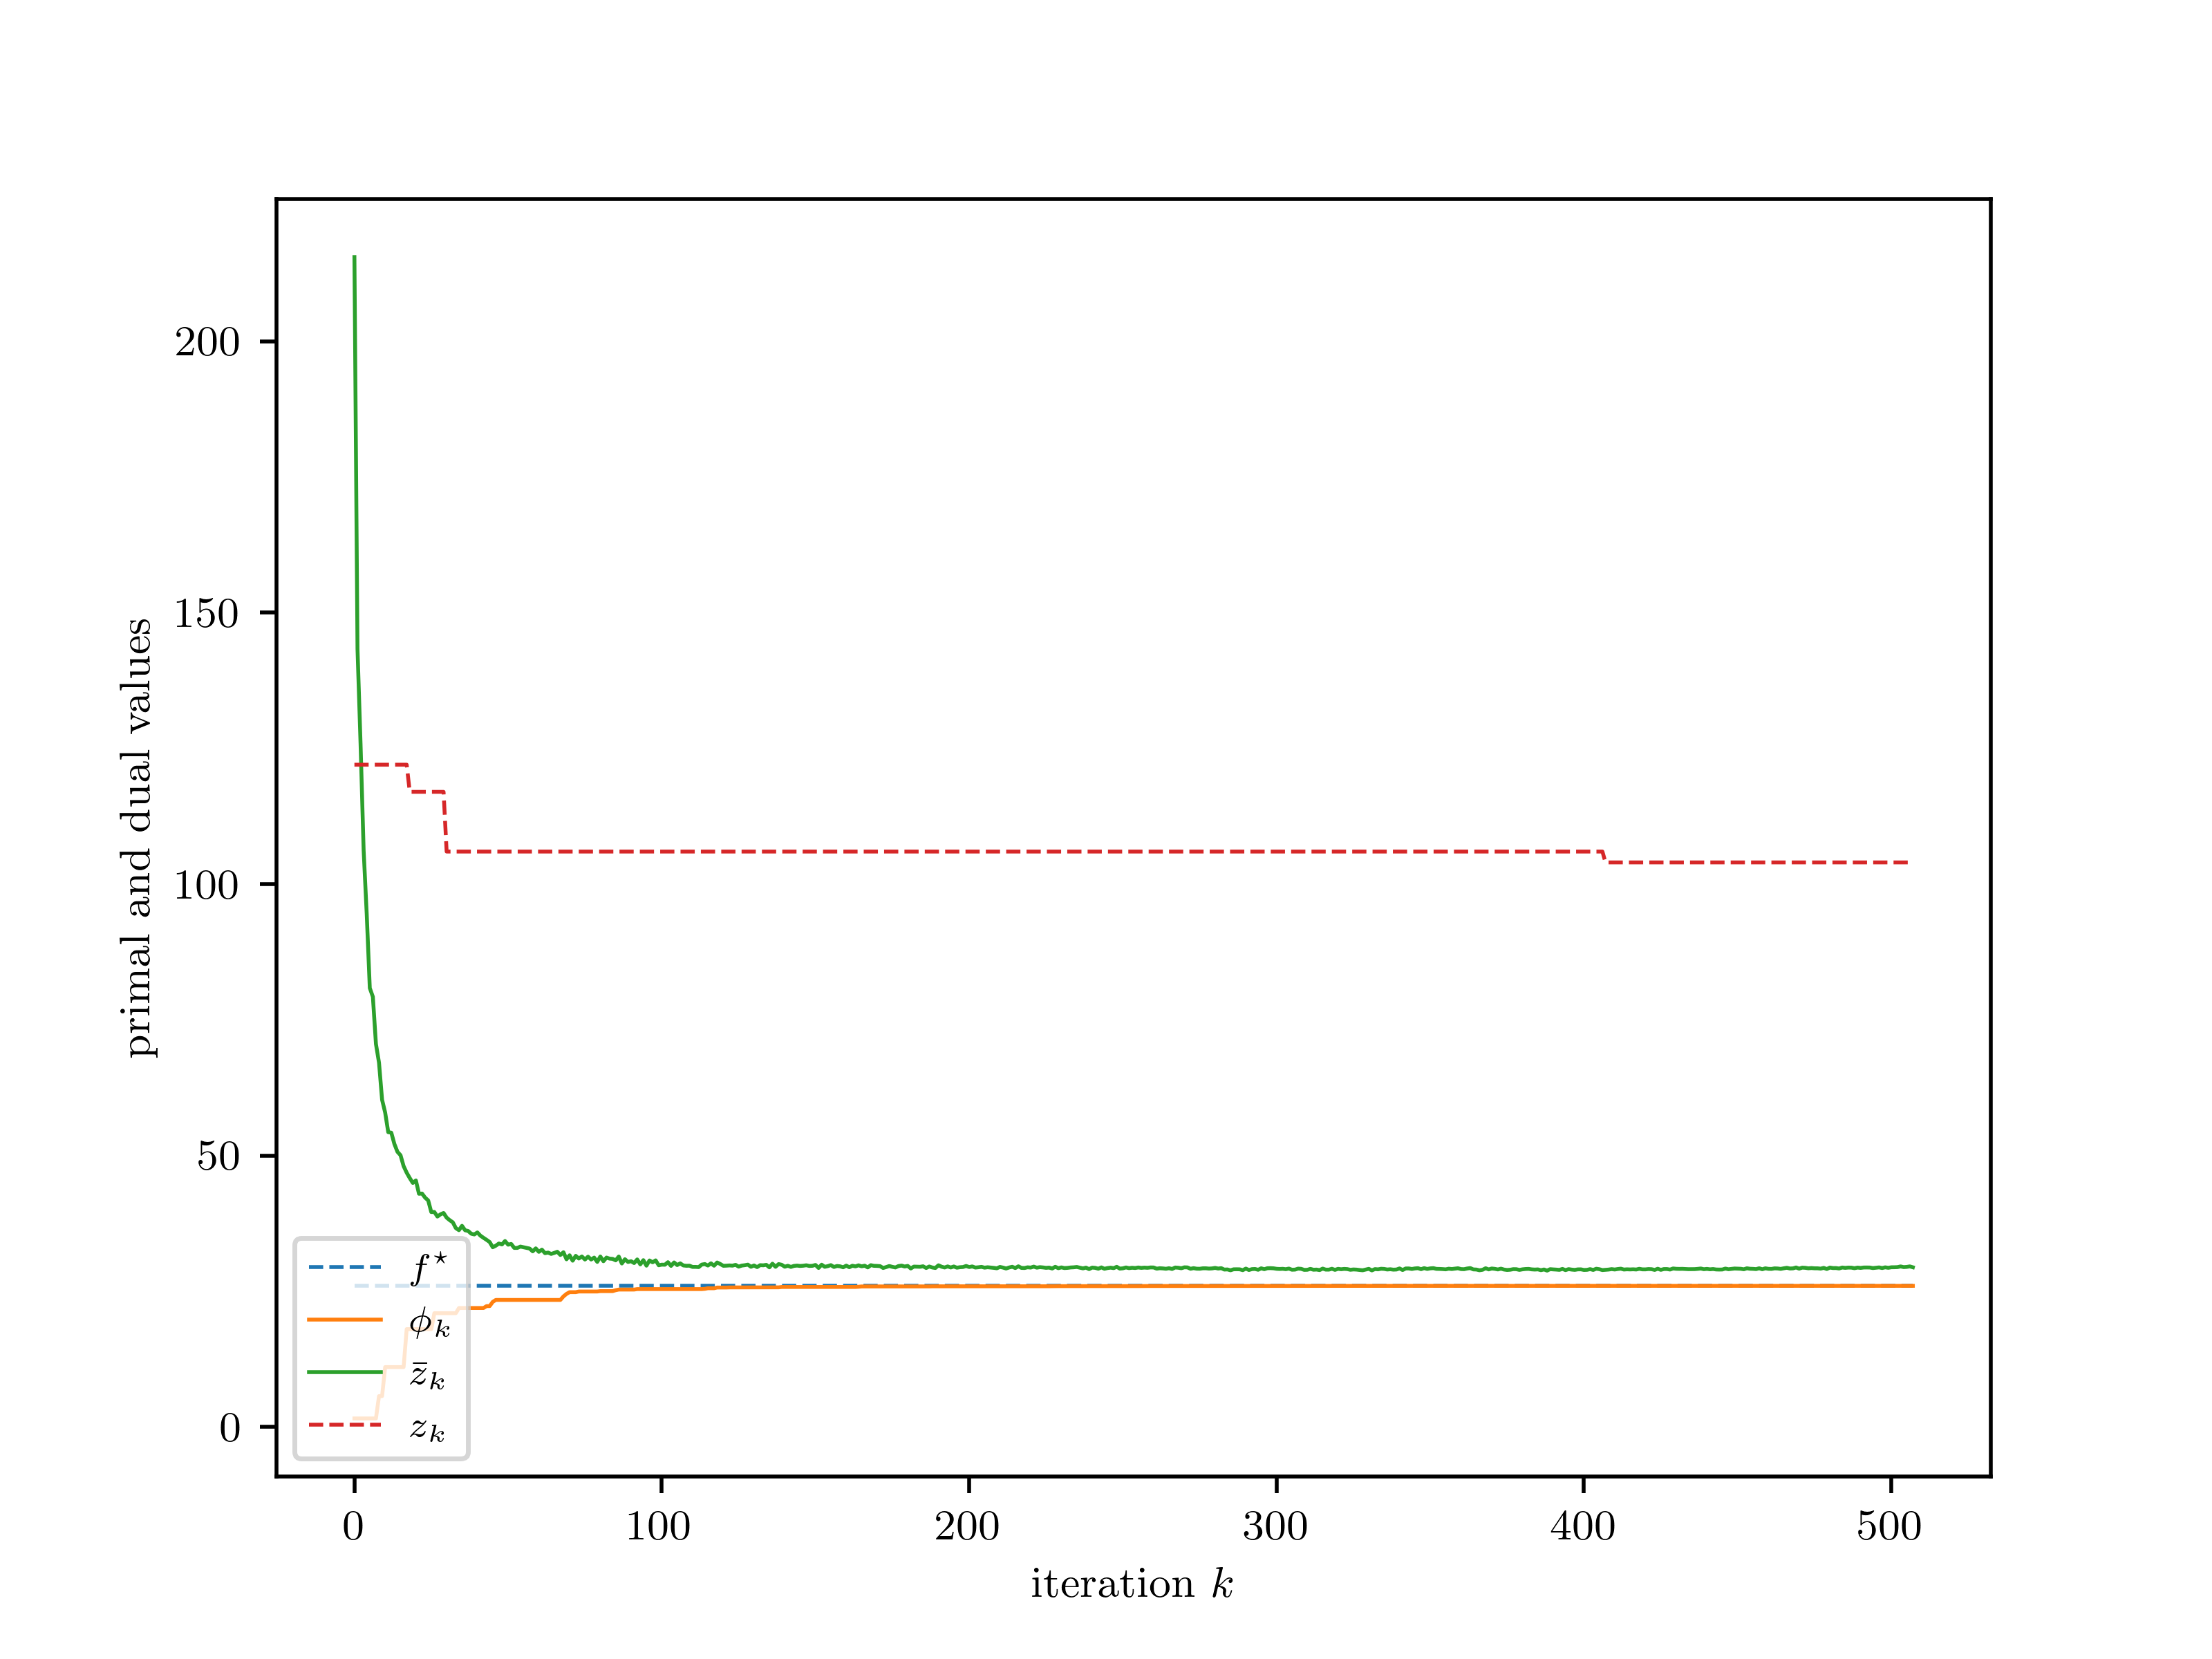
\includegraphics[width=.89\linewidth]{imgs/conv_0_normal_sg_10_15.png}

    \label{fig:divergent_volume}
  \end{figure}
\end{frame}

\begin{frame}
  \frametitle{FMP: \(c \neq 1\) small case \(5 \times 5\)}
  \scriptsize
  \begin{tabular}{lllrrrlllll}
    \toprule
    {} & lb\_grb & \(f_{\textsf{grb}}\)   & t\_grb
       & t\_sg   & \(\phi_{\textsf{sg}}\) & \(\phi_{\textsf{gap}}\)                            \\
    %  & \( z_{\textsf{sg}}\) & z\_gap                                                                                                                                      \\
    \midrule
    0  & 0.00    & 0.00                   & 0.00                    & 0.00 & 0.00  & 0.00\%    \\
    1  & 16.00   & 16.00                  & 0.01                    & 1.22 & 6.00  & -62.50\%  \\
    2  & 0.00    & 0.00                   & 0.03                    & 1.92 & -0.00 & -120.00\% \\
    3  & 6.00    & 6.00                   & 0.02                    & 1.05 & 4.00  & -33.33\%  \\
    4  & 16.00   & 16.00                  & 0.04                    & 1.14 & 16.00 & -0.00\%   \\
    5  & 0.00    & 0.00                   & 0.01                    & 1.25 & -0.00 & -80.00\%  \\
    6  & 5.00    & 5.00                   & 0.01                    & 1.53 & 3.00  & -40.00\%  \\
    7  & 5.00    & 5.00                   & 0.02                    & 1.49 & 4.00  & -20.00\%  \\
    8  & 0.00    & 0.00                   & 0.01                    & 1.53 & -0.00 & -70.00\%  \\
    9  & 0.00    & 0.00                   & 0.02                    & 1.48 & -0.00 & -50.00\%  \\
    10 & 17.00   & 17.00                  & 0.02                    & 1.15 & 14.00 & -17.65\%  \\
    11 & 5.00    & 5.00                   & 0.06                    & 1.32 & -0.00 & -99.99\%  \\
    12 & 1.00    & 1.00                   & 0.03                    & 1.19 & -0.00 & -100.02\% \\
    13 & 8.00    & 8.00                   & 0.02                    & 1.06 & 8.00  & -0.01\%   \\
    14 & 12.00   & 12.00                  & 0.02                    & 0.98 & 12.00 & -0.00\%   \\
    15 & 4.00    & 4.00                   & 0.02                    & 1.02 & -0.00 & -99.99\%  \\
    16 & 2.00    & 2.00                   & 0.03                    & 1.70 & -0.00 & -99.99\%  \\
    17 & 0.00    & 0.00                   & 0.01                    & 1.23 & -0.00 & -70.00\%  \\
    18 & 0.00    & 0.00                   & 0.01                    & 1.28 & -0.00 & -60.00\%  \\
    19 & 2.00    & 2.00                   & 0.01                    & 1.16 & -0.00 & -99.99\%  \\
    20 & 0.00    & 0.00                   & 0.02                    & 1.38 & -0.00 & -70.00\%  \\
    \bottomrule
    \normalsize
  \end{tabular}
\end{frame}

\begin{frame}
  \frametitle{Conclusion}

  \begin{itemize}
    \item ? zero duality gap: \(\phi^\star = f^\star\), \(\phi^\star\) is the best bound by \(\phi\) and \( f^\star\) is the best primal value.
    \item ? can we bound the quality of heuristic for averaged solution? \(\bar z_k = z(\bar y_k)\) converges to \(\phi^\star\):
          \[|\bar z_k - \phi^\star| \]
    \item can we improve \(\bar z = z(\bar y)\)? round \(\bar z\)
  \end{itemize}
\end{frame}

\end{document}
